\documentclass[conference]{IEEEtran}
\IEEEoverridecommandlockouts

\usepackage{amsmath,amssymb,amsfonts}
\usepackage[english]{babel}
\usepackage{algorithmic}
\usepackage{multicol}
\usepackage{booktabs}
\usepackage{graphicx}
\usepackage{textcomp}
\usepackage{xcolor}
\usepackage{array}
\usepackage{cite}
\usepackage{url}

\def\BibTeX{{\rm B\kern-.05em{\sc i\kern-.025em b}\kern-.08em
    T\kern-.1667em\lower.7ex\hbox{E}\kern-.125emX}}
\begin{document}

\title{Securing Data in Low-Resource Environments: Lightweight Block Ciphers}


\author{\IEEEauthorblockN{Fernando Ramirez Arredondo}
\IEEEauthorblockA{\textit{Computer Science} \\
\textit{Universidad Católica San Pablo}\\
Arequipa, Perú \\
fernando.ramirez@ucsp.edu.pe}
\and
\IEEEauthorblockN{Yván Jesús Túpac Valdivia}
\IEEEauthorblockA{\textit{Computer Science} \\
\textit{Universidad Católica San Pablo}\\
Arequipa, Perú \\
ytupac@ucsp.edu.pe}}


\maketitle

\begin{abstract}
    Ensuring communication security for devices with limited resources is vital in the contemporary landscape. This work classifies seven state-of-the-art lightweight block ciphers designed for such devices. These ciphers offer efficient encryption for data security while minimizing resource consumption. This work focuses on the two main categories of lightweight block ciphers, Substitution-Permutation Networks and Feistel Networks. The experiments reveals that Feistel Networks excel with limited resources and when decryption implementation is needed, while Substitution-Permutation Networks excel at execution time.
\end{abstract}

\begin{IEEEkeywords}
iot, feistel, substitution-permutation, resource-constrained, lightweight, cryptography
\end{IEEEkeywords}

\section{Introduction}\label{sec:intro}

The development of Internet of Things (IoT) technology started an era of interconnected devices, collecting data from the physical world and transforming our interaction with it. This connectivity presents a security challenge when the devices generating or transmitting sensitive data lack the resources to perform up-to-standard encryption processes. As Thakor et al. \cite{IoT_1} categorize, IoT devices fall into two resource-based groups, resource-rich devices like servers, personal computers, and smartphones, and resource-constrained devices like sensor nodes, radio-frequency identification (RFID) tags, and actuators. See Table \ref{table:crypto_devices} for the categorization.

\begin{table}[ht]
    \centering
    \caption{Cryptographic Approaches on Different Devices\cite{IoT_1}}
    \begin{tabular}{ll}
        \toprule
        \textbf{Device} & \textbf{Cryptography} \\
        \midrule
        Servers, Desktops and Smartphones & Conventional Cryptography \\
        Embedded Systems and RFID & Lightweight Cryptography \\
        \bottomrule
    \end{tabular}
    \label{table:crypto_devices}
\end{table}

This challenge is further amplified by the evolution of IoT, which has transitioned from smaller networks to wide area networks, leading to a rapid growth in the number of interconnected devices. As IoT applications increase, a substantial amount of sensitive data is exchanged, raising concerns about privacy and security. Increased device interconnectivity further intensifies these concerns, potentially exposing new vulnerabilities with each additional device. In a landscape with billions of interconnected devices, a single security flaw can be exploited on a massive scale.
Just as physical security measures like locks, safes, and opaque envelopes protect our valuables, cryptography serves as the digital equivalent, safeguarding the integrity and confidentiality of data in our online activities. This work aims to contribute to the application of cryptography for resource-constrained devices in the ever-expanding IoT landscape, where robust security solutions are essential to trust the activities and processes we reproduce or create from scratch in the digital world. 

Traditional cryptography, often computationally intensive, is impractical for resource-constrained devices. Lightweight cryptography emerges as a modern solution, specifically designed for devices with limitations in memory, processing power, and energy consumption. It prioritizes low computational complexity and a small memory footprint\cite{zhong2024lightweight}. Ciphers are divided into two main categories, asymmetric and symmetric. While asymmetric ciphers offer enhanced security features, they require greater computational resources and often have higher implementation costs. Consequently, they are less suitable for resource-constrained devices. Lightweight ciphers lean into the symmetric approach due to being generally faster and requiring less computational power. Following this same line of thinking, the vast majority of these ciphers are designed to operate on fixed-sized blocks of data rather than streams of data, as can be seen in NIST latest Lightweight Cryptography Standardization Process\cite{NIST}. It is for this reasons that this study focuses on block ciphers, specifically on two fundamental structures employed in lightweight block ciphers (LBC), Feistel Network (FN) and Substitution-Permutation Network (SPN).

\begin{figure*}
    \centering
    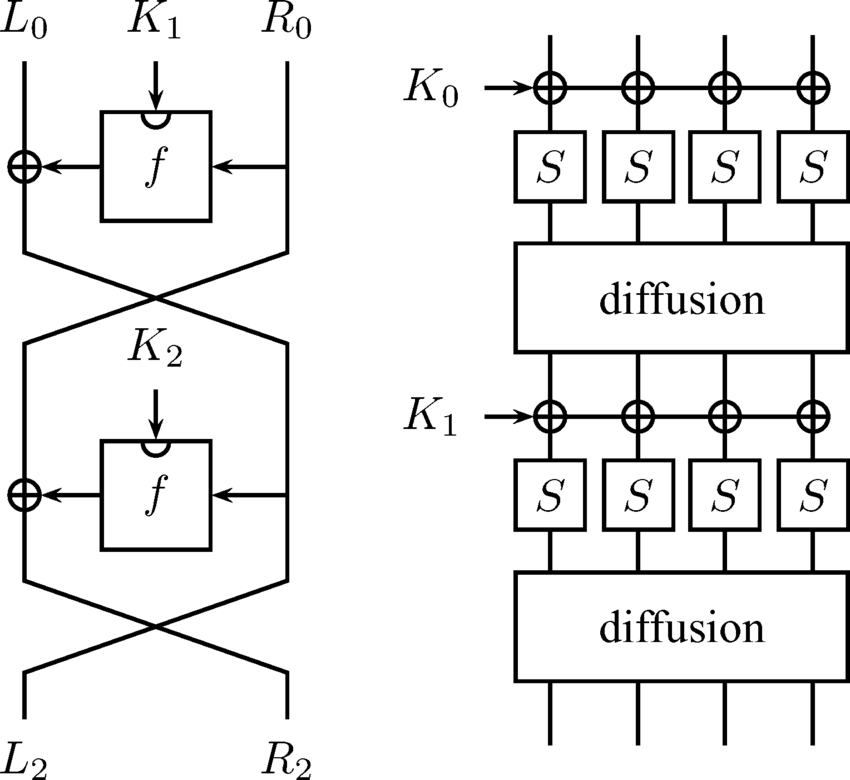
\includegraphics[width=\columnwidth]{figures/FEISTEL-SPN.png}
    \caption{Generalization of a Feistel Network (left) and a Substitution-Permutation Network (right)\cite{de2006introduction}.}
    \label{fig:FEISTEL-SPN}
\end{figure*}

The Feistel Network offers a modular and efficient approach to encryption, employing multiple rounds of data processing. In each round, a half-block of data is processed using a round function, often incorporating non-linear substitutions and permutations (operations do not follow a simple proportional relationship). The output of this function is then combined with the other half-block using an XOR operation, creating a dependency between rounds that improves the overall security\cite{FEISTEL}.

The Substitution-Permutation Network relies on a series of substitution and permutation stages. Substitution box (S-box) replaces data bits, introducing non-linearity to confuse potential attackers. Permutation box (P-box) rearranges the data bits, making it challenging to discern the original data\cite{heys1996substitution}. Refer to Fig.\ref{fig:FEISTEL-SPN} for a general view of both FN and SPN structures.

Both FN and SPN structures offer advantages in lightweight cryptography. FN structures are known for their modularity and ease of implementation, while SPN structures provide inherent parallelism, potentially leading to faster encryption/decryption on certain architectures.
This paper makes an exploration of FN and SPN structures in the context of lightweight cryptography. We will provide analysis of their design principles, operational workflows, and suitability for resource-constrained devices.

Section \ref{sec:art}.
Section \ref{sec:tec}.
Section \ref{sec:imp}.
Section \ref{sec:exp}.
Section \ref{sec:conc}.

\section{State of the art}\label{sec:art}

This section explores lightweight block ciphers, introducing them based on their structure and the techniques that generate their state-of-the-art performance for resource-constrained devices.

\subsection{SPN-based solutions}

Dynamic Ultra-Lightweight Block Cipher (DULBC) employs a dynamic SPN structure in which the specific encryption process changes based on the round keys, generating a non-fixed round function. Each round selects one of four functions ($f$s) based on the first two bits of the round key, enhancing security without significant hardware overhead. The proposed S-box consists of three NOR and XOR, one NAND and XNOR operations, leading to a simple inverse and efficient implementation and good cryptographic properties with minimal cost. The authors highlight successful Field Programmable Gate Array (FPGA) and Application-Specific Integrated Circuit (ASIC) implementations of DULBC, demonstrating high throughput (number of operations processed per unit time) and relatively low area requirements (number of transistors needed to build the hardware that performs the encryption operations). Security analysis confirms the resistance of DULBC to various attacks, including differential attacks, linear attacks, and side-channel attacks.


Yasmin and Gupta proposed a modification to the LBC GIFT\cite{GIFT}. The main focus is on improving diffusion, how a single bit change in the message spreads throughout the ciphertext. It improves upon the original GIFT by enhancing the Key Scheduling Algorithm (KSA) using bit-slicing substitution and involutive permutation. By operating on multiple bits at once, in bit-slicing substitution, the larger data element is sliced into smaller pieces. Each slice is then independently subjected to the substitution operation using the S-box. This enables the concurrent processing of multiple bits at once, leveraging the architecture of the processor. By shuffling the bits and then applying the inverse permutation later, the original bit positions are obscured, making it harder to track how changes in the plaintext affect the ciphertext, leading to better diffusion and randomness in round keys. This addresses the predictability issue of the original KSA\cite{yasmin2023modified}.


InVolutive Lightweight Block Cipher (IVLBC) is LBC designed for unified encryption-decryption in resource-limited environments. The design prioritizes high diffusion (influence of a single bit change in the plaintext over the ciphertext) for strong encryption, involution (components return to their original state after two applications) for efficient implementation and flexibility in hardware and software implementations. To achieve these goals, IVLBC utilizes a FN structure with a tree-based design for a compact and efficient S-box, by using a tree-based structure with logic operations, the S-box in IVLBC can achieve the same functionality as a traditional table-based S-box while requiring less memory and potentially faster processing. Additionally, it employs a unique nibble-based involutive permutation to enhance diffusion. Using nibble-based operations can further enhance diffusion by disrupting patterns across larger chunks of data compared to single-bit permutations. Decryption can reuse the same circuitry as encryption, leading to lower resource requirements\cite{IVLBC}.

\subsection{FN-based solutions}

SCENERY is a LBC that makes use of bit-slicing in the round function design to achieve low-cost hardware and efficient software implementations. Bit-slicing is a technique that operates each bit of the data block in a separate, smaller unit called a slice, rather than working with entire blocks. The main benefits of this implementation are speed improvements on hardware that supports parallel execution and simpler logic circuits in hardware design, potentially reducing area and power consumption compared to traditional designs. While bit-slicing increases code complexity, lightweight ciphers are not complex by definition, so this is not a significant issue if executed correctly. To address the slow diffusion issue that can occur with a FN, SCENERY incorporates a 32x32 binary matrix used to operate in the 64-bit blocks that can be implemented efficiently and improves diffusion speed. The authors propose a new Key Scheduling Algorithm (KSA) to tackle the issue of backward derivation of the master key. While not a complete solution, this method makes it more difficult compared to the key scheduling of PRESENT\cite{PRESENT} and enhances the security of key expansion.\cite{SCENERY}


Lightweight Block encryption algorithm based on Combined Chaotic System (LBCSS) is a LBC that uses a combined chaotic system for encryption and decryption. This means that instead of relying on a single mathematical function that exhibit chaotic behavior, LBCSS uses multiple functions together. This chaotic system is used to create secure S-boxes, P-boxes, and keys for the encryption process. LBCSS makes use a structure that enhances diffusion compared to the traditional FN, but maintains a concise design. The round function is created using bit-slicing techniques. Operations like substitutions, rotations, or bitwise operations introduce non-linear transformations on the data. These operations ensure a complex relationship between the plaintext and the ciphertext. The round function remains consistent across all encryption rounds to maintain low complexity. To prevent these consistent rounds from becoming too predictable, round constants are introduced to add variation. The authors argue that LBCSS offers sufficient security based on various tests, including resistance to different cryptanalysis methods and statistical testing.\cite{LBCCS}


SAND is a LBC that it employs AND, Rotation, and XOR operations (AND-RX) within a FN. Traditionally, evaluating the security of AND-RX ciphers can be complex because these operations often work on individual bits within the data, making it difficult to apply existing analysis methods typically used for S-boxes. SAND allows for easier security evaluation compared to other AND-RX ciphers by utilizing AND-RX operations within small data units (nibbles). This allows security researchers to use existing methods designed for analyzing S-boxes, which are a more familiar and well-studied component in cryptography. The authors highlight the benefits of SAND in terms of both security and performance. SAND achieves strong security under various attack scenarios, including differential and linear attacks. The paper also discusses the motivations behind the design of SAND. Existing ARX-based ciphers often rely on large S-boxes, which are not ideal for hardware implementation. SAND provides an AND-RX design with efficient hardware implementation and strong security guarantees through its novel S-box transformation approach.\cite{SAND}


LBC-IoT achieves diffusion by employing a combination of techniques, including a compact S-box with high non-linearity properties for data substitution and dedicated P-boxes for bit permutation, further obfuscating the relationship between the original and encrypted data. It is well known that FN structures can lack diffusion due to the round function $f$ being applied to only half of the data each round. The solution of LBC-IoT to this problem is to apply a different P-box to each half of the data at the end of the rounds. The cipher utilizes simple operations within its core function and keeps the S-box size small. This approach minimizes the amount of processing power and memory required for implementation. Security-wise, LBC-IoT is resistant to brute-force attacks by adhering to NIST recommendations for key length. It uses an 80-bit key, which is too complex to crack through exhaustive searching methods. The authors ensure that LBC-IoT offers a good balance between robust security and efficient implementation.\cite{LBC-IoT}

\begin{table*}[ht]
    \centering
    \caption{Lightweight Block Ciphers}
    \begin{tabular}{lllll} 
     \toprule
     Algorithm & Key size & Block size & N. of rounds & Structure \\ 
     \midrule
     DULBC (Yang et al., 2022) \cite{DULBC} & 80/128 & 64 & 25/30 & SPN \\
     GIFT (Yasmin and Gupta, 2023)\cite{GIFT}\cite{yasmin2023modified} & 128 & 64/128 & 28/40 & SPN \\
     IVLBC (Huang et al., 2023)\cite{IVLBC} & 80/128 & 64 & 29 & SPN \\
     LBC-IoT (Ramadan et al., 2021)\cite{LBC-IoT} & 80 & 32 & 32 & Feistel  \\
     SAND (Chen et al., 2021)\cite{SAND} & 128 & 64/128 & 48/54 & Feistel \\
     LBCCS (Zhu et al., 2022)\cite{LBCCS} & 128 & 128 & 20 & Feistel \\
     SCENERY (Feng and Li et al., 2022)\cite{SCENERY} & 80 & 64 & 28 & Feistel  \\
     \bottomrule
    \end{tabular}
    \label{table:ciphers}
\end{table*}

Lightweight block ciphers are categorized based on their genereal metrics and structure. The performance of each algorithm is evaluated based on the following metrics.
\begin{itemize}
    \item \textbf{Block Size}: To save on processing power and battery life in IoT devices, block ciphers chop up the data they encrypt into small, pre-defined chunks. The size of these chunks directly impacts how much energy the encryption process consumes. As shown in Table \ref{table:ciphers}, GIFT, SAND and LBCCS have the largest block size of 128 bits while LBC-IoT adopts the smallest block size of only 32 bits. Most surveyed ciphers employ 64-bit blocks.
    \item \textbf{Key Size}: The number of bits in a cryptographic key, known as the key size, directly affects security. Bigger keys are like more complex locks, offering stronger protection however, they require more effort (processing power and energy) to use. NIST suggests a minimum key size of 80 bits for basic defense against brute-force attacks, where attackers try every possible key combination\cite{barker2018transitioning}. Reflecting this trade-off, none of the ciphers in Table \ref{table:ciphers} exceed 128 bits or fall below 80 bits, opting for one of these two key sizes.
    \item \textbf{Number of rounds}: Compared to conventional ciphers, lightweight block ciphers prioritize simplicity to work on devices with limited resources. Unlike conventional ciphers, they achieve strong security through multiple rounds of processing. While each extra round makes the cipher harder to crack, it also slows down the encryption process. This approach ensures that breaking the cipher becomes more effort than simply trying every possible key.
\end{itemize}

\section{Techniques to implement}\label{sec:tec}

This section goes deeper into two of the lightweight block cipher techniques introduced earlier, SAND and GIFT. The remainder of this section will outline their encryption and decryption processes, along with the rationale behind chosing them for implementation. NOTE: Implementations will follow NIST Recommendation for Block Cipher Modes of Operation\cite{dworkin2001recommendation}.

\subsection{GIFT}

GIFT comes in two variants, GIFT-64, a 64-bit block size, 28-round SPN cipher, and GIFT-128, a 128-bit block size, 40-round SPN cipher. Due to its larger block size offering potentially stronger security, GIFT-128 will be implemented for this project\cite{yasmin2023modified}.

\subsubsection{Structure for encryption and decryption}

This cipher operates in rounds, with each round consisting of five steps, S-box generation, bitslice substitution, involutive permutation, addition of the round key, and a constant XOR. The decryption process consists of performing the same steps with inversed P-box and S-box. The complete KSA and the processes of encryption and decryption followed in the GIFT cipher can be found in the original proposal by Banik et al\cite{GIFT}. However, Yasmin and Gupta enhanced the cipher by incorporating bitslice substitution and an involutive permutation\cite{yasmin2023modified}. Refer to Fig.\ref{fig:GIFT-} for a representation of the round function.

\begin{figure}
    \centering
    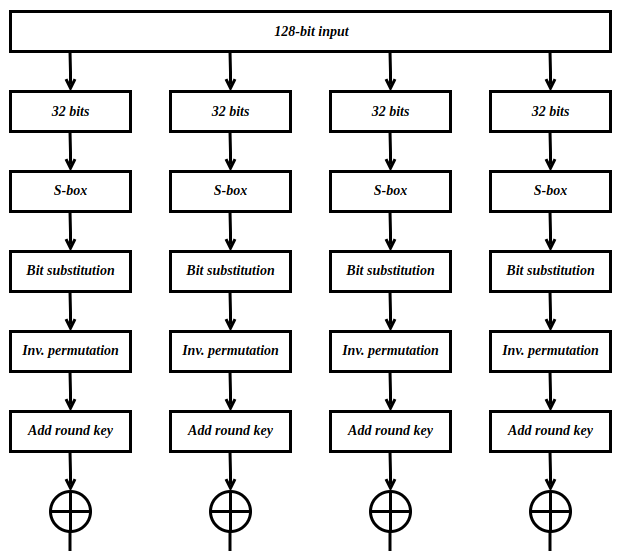
\includegraphics[width=0.8\columnwidth]{figures/GIFT-ROUND.png}
    \caption{Representation of the encryption round function of GIFT\cite{yasmin2023modified}.}
    \label{fig:GIFT-}
\end{figure}

\subsubsection{Reasons for implementation}

The GIFT block cipher, known for its efficiency, has traditionally relied on linear functions within its KSA. However, this approach exhibits vulnerabilities, potentially leading to diminished performance and the predictability of bit transitions. This novel iteration of GIFT proposes the incorporation of bitslice substitution and involutive permutation operations to improve the randomness and diffusion characteristics. These security enhancements to a well-regarded cipher appear to be a promising advancement.

\subsection{SAND}
SAND is a family of two AND-RX block ciphers with Feistel structure, SAND-64, a 64-bit block size, 48-round cipher, and SAND-128, a 128-bit block size, 54-round cipher. Due to its larger block size offering potentially stronger security, SAND-128 will be implemented for this project\cite{SAND}.
\subsubsection{Structure for encryption and decryption}
The round function of the SAND cipher depends on a mix of AND, rotation, and XOR operations. Following the principle of expand-then-compress, the left input branch expands into two branches to facilitate parallel confusion and diffusion within the round function. Each round consists of constant rotation, non-linear functions, bit permutation, an XOR operation with the right input, and the addition of the round key. The decryption process is very similar to encryption, but the round keys are applied in reverse order. This allows the network to reverse the operations performed during encryption and recover the original data. For a detailed breakdown of the encryption process and the complete KSA, refer to the original proposal by Chen et al\cite{SAND}. Refer to Fig.\ref{fig:SAND-} for a representation of the round function.

\begin{figure}
    \centering
    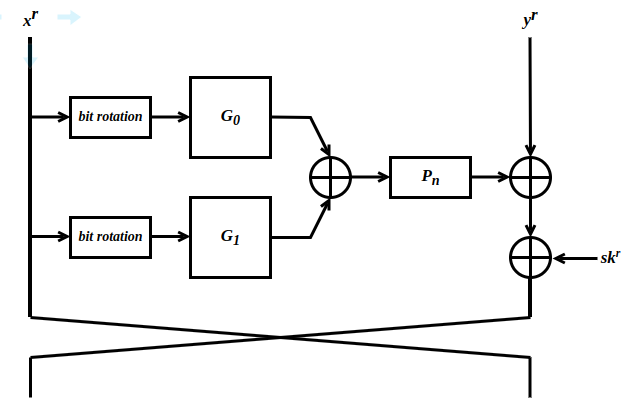
\includegraphics[width=0.9\columnwidth]{figures/SAND-ROUND.png}
    \caption{Representation of the encryption round function of SAND\cite{SAND}.}
    \label{fig:SAND-}
\end{figure}


\subsubsection{Reasons for implementation}
SAND leverages a novel design approach that restricts its AND-RX operations to work within 4-bit nibbles. This unique approach allows SAND to be represented equivalently using a 4x8 synthetic S-box (SSb). This conversion unlocks the advantage of employing established S-box-based security evaluation methods. Furthermore, the authors claim that the inherent bitslice structure combined with AND-RX operations positions SAND among the top contenders for efficient software implementation. The simplicity of employing AND-RX operations and the robustness of well-developed S-box-based security evalution methods and tools appear to be a promising advancement.

\section{Implementation}\label{sec:imp}

This section details the implementation of the SAND-128 and GIFT-128 lightweight ciphers in software. The source code is writen out in C. The metrics used to judge the performance of the implementations are execution time, code size, memory usage, total cycles, latency, efficiency, and throughput, plus a synthetic metric. The rest of the section describes the process and key considerations for the software implementation.

\subsection{Algorithm Specification and Code Development}

The specifications of SAND-128 and GIFT-128 were studied from their respective academic papers. Using the algorithm specifications, the encryption and decryption functions for both ciphers were implemented in C.

\begin{verbatim}
// GIFT-128 encryption function
void GIFT128_ENC(uint8_t plaintext[16],
                 uint8_t key[16],
                 uint8_t ciphertext[16]){
    // Initialization and key schedule
    // Perform encryption rounds
    // Output ciphertext
}
//
\end{verbatim}

\subsection{Testing and Validation}

The implemented C code was tested against the test vectors in NIST Special Publication 800-38A 2001 ED\cite{dworkin2001recommendation}, which provides recommendations for block cipher modes of operation. The selected encryption mode is the electronic codebook (ECB). The main drawback lies in its limited diffusion capability, as it does not effectively conceal data patterns when encrypting identical plaintext blocks, resulting in identical ciphertext blocks. This critical disadvantage can be ignored when the plaintext blocks are selected in a testing environment, leaving ECB as the optimal encryption mode because of its simplicity. These tests ensured that the software implementation produced correct outputs for known inputs.

\begin{verbatim}
// NIST test vectors
plain-text:
    6bc1bee22e409f96e93d7e117393172a
    ae2d8a571e03ac9c9eb76fac45af8e51
    30c81c46a35ce411e5fbc1191a0a52ef
    f69f2445df4f9b17ad2b417be66c3710
key:
    2b7e151628aed2a6abf7158809cf4f3c
//
\end{verbatim}

\subsection{Performance Evaluation}

The performance of the software implementation was evaluated based on the following metrics.

\begin{itemize}
    \item \textbf{Execution Time}: The time taken to perform encryption operations was measured using high-resolution timers.
    \item \textbf{Code Size}: Memory size to store the cipher code and constants, measured in kilobytes ($\text{kB}$).
    \item \textbf{Memory Usage}: The memory consumption during the encryption process was analyzed for both RAM and ROM.
    \item \textbf{Throughput}: The number of operations processed per unit time was calculated to determine the efficiency of the implementation. Throughput, denoted as \( T \), can be defined as:
    \[ T = \frac{D}{s} \]
    where \( D \) is the data size in megabytes (MB) and \( s \) is the time in seconds or as \( t \):
    \[ t = \frac{d}{ms} \]
    where \( d \) is the data size in kilobits (kb) and \( ms \) is the time in milliseconds.
    \item \textbf{Total Cycles}: The total number of clock cycles required for the encryption process.
    \item \textbf{Latency}: Latency denotes the number of clock cycles required to compute each plaintext/ciphertext block. Latency, denoted as \( L \), can be defined as:
    \[ L = \frac{N_b}{C} \]
    where \( N_b \) is the number of 128-bit blocks and \( C \) is the number of cycles.
    \item \textbf{Efficiency}: Efficiency evaluates the relationship between performance and implementation cost. Generally, higher efficiency values are preferable. Software efficiency follows.
    \[ E = \frac{t}{S} \]
    where \( t \) is throughput in kilobits per second (kbps) and \( S \) is the code size in kilobytes (kB).
    \item \textbf{Synthetic Metrics}: A combined metric such as Code Size $\times$ Cycle Count $/$ Block Size.
\end{itemize}

\section{Experiments and Results}\label{sec:exp}

\begin{table*}[ht]
  \centering
  \caption{Comparison of software performance for encryption with 2MB of messages.}
  \begin{tabular}{lllllllll} 
   \toprule
   Algorithm & Execution Time & Code Size & Memory Usage & Throughput & Total Cycles & Latency & Efficiency & Synth. Metric\\ 
   \midrule
   GIFT-128 & 47309 ms & 12.5 kB & 23.2 kB & 21.14 & 162842486 & 1242 & 13852.76 & 15902587 \\
   SAND-128 & 130976 ms & 4.6 kB & 9 kB & 15.27 & 452417454 & 3452 & 27193.83 & 16258752  \\
   \bottomrule
  \end{tabular}
  \label{table:enc}
\end{table*}

In this experiments, the key schedule is not taken into account as the round keys are assumed to be precomputed and stored in RAM. The benchmark consists in measuring the time required to encrypt and decryption 2MB data using the ECB mode. All benchmarking results can be found in Table \ref{table:enc} \& \ref{table:dec} and all the tests are accomplished on a PC with 2.7GHz Intel(R) Core i7-7500U CPU using gcc 13.2.0.  

It can be observed that the GIFT-128 execution time is almost three times shorter than the SAND-128 execution time. This can be attributed in part to the number of rounds and the complexity of functions. The code size is 12.5 kB for GIFT-128 and 4.6 kB for SAND-128. This metric is important when implementation space is limited and code size needs to be minimal. It is important to note that the code size of GIFT will inevitably increase if decryption is also implemented, while the SAND code size will remain the same. Memory usage is significantly smaller for SAND-128, which is crucial when resources are limited and memory usage must be minimal. Throughput, referring to the MB of data processed per second, is better for GIFT-128 at 21.14 MB/s compared to SAND-128 15.27 MB/s. In terms of clock cycles, GIFT-128 employs 1242 cycles per 128-bit block of data, while SAND-128 uses 3452 cycles per 128-bit block of data. Efficiency evaluates the relationship between performance and implementation cost in terms of throughput and code size; SAND-128 is almost twice as efficient as GIFT-128. The synthetic metric reveals that even though these ciphers operate in very distinct ways, considering the previously mentioned metrics, their performance is very similar in terms of code size and cycles per block.

\begin{table*}[ht]
  \centering
  \caption{Comparison of software performance for encryption and decryption with 2MB of messages.}
  \begin{tabular}{lllllllll} 
   \toprule
   Algorithm & Execution Time & Code Size & Memory Usage & Throughput & Total Cycles & Latency & Efficiency & Synth. Metric\\ 
   \midrule
   GIFT-128 & 0 & 0 & 0 & 0 & 0 & 0 & 0 & 0 \\
   SAND-128 & 0 & 0 & 0 & 0 & 0 & 0 & 0 & 0  \\
   \bottomrule
  \end{tabular}
  \label{table:dec}
\end{table*}


\section{Conclusions}\label{sec:conc}
Feistel networks and Substitution-Permutation networks are both fundamental structures for designing lightweight block ciphers. While they share some similarities, they have distinct advantages and disadvantages.

Feistel networks offer invertibility, meaning decryption is straightforward even if the round function itself is not invertible. This simplifies design and analysis. However, these ciphers also have drawbacks. The overall security depends heavily on a strong Feistel function, and each round introduces processing overhead, potentially slowing down encryption and decryption.

Substitution-Permutation networks can achieve higher throughput due to their inherent parallelism, making them attractive for implementations with multiple processing units, and confusion by employing S-boxes that perform non-linear operations on the data, making the link between plaintext, key, and ciphertext highly complex. Additionally, P-boxes ensure diffusion by rearranging the data bits, such that a single change in the plaintext has a cascading effect on the final ciphertext. Ultimately, the number of encryption rounds and the design of the S-boxes and P-boxes play a critical role in determining the strength and security of an Substitution-Permutation network cipher.

Making the best choice between a Feistel network and a Substitution-Permutation network depends on the specific application and design goals. If ease of decryption and hardware limitations are key concerns, a Feistel network might be preferable. If maximizing encryption speed on parallel hardware is a priority, a Substitution-Permutation network might be a better choice.

Bit-slicing allows for parallel processing on hardware that supports it, potentially leading to significant speed improvements. It is particularly beneficial for lightweight ciphers designed for resource-constrained environments. However, bit-slicing can increase code complexity, so it is important to find a balance between efficiency and implementation effort. Some S-boxes might be designed with low complexity for compact hardware implementations, while others might prioritize high non-linearity for enhanced security.

The development of lightweight cryptography seems to be a continuing search for balance between security and efficiency. On one hand, lightweight ciphers need to be strong enough to resist attacks, but on the other hand, they must also be efficient in terms of resource consumption (memory, processing power) to run on devices with limited capabilities.


\bibliographystyle{IEEEtran}
\bibliography{bibliography/references}
\vspace{12pt}

\end{document}
